% Template:     Template Tesis LaTeX
% Documento:    Archivo principal
% Versión:      1.1.7 (02/10/2019)
% Codificación: UTF-8
%
% Autor: Pablo Pizarro R. @ppizarror
%        Facultad de Ciencias Físicas y Matemáticas
%        Universidad de Chile
%        pablo.pizarro@ing.uchile.cl, ppizarror.com
%
% Sitio web:    [https://latex.ppizarror.com/tesis]
% Licencia MIT: [https://opensource.org/licenses/MIT]
% CREACIÓN DEL DOCUMENTO
\documentclass[letterpaper,12pt,oneside]{book} % Libro, tamaño carta
\usepackage[utf8]{inputenc} % Codificación UTF-8

\bibliographystyle{unsrtnat}
% INFORMACIÓN DEL DOCUMENTO
\def\titulotesis {Modelamiento y seguimiento de tópicos para detección de modus operandi en robo de vehículos}
\def\titulogrado {
	Tesis para optar al grado de magíster en gestión de operaciones
	\bigbreak\vspace{0.3cm}
	Memoria para optar al título de ingeniero civil industrial
}

\def\nombreuniversidad {Universidad de Chile}
\def\nombrefacultad {Facultad de Ciencias Físicas y Matemáticas}
\def\departamentouniversidad {Departamento de Ingeniería Industrial}
\def\imagendepartamento {img/dptos/uchile2.pdf}
\def\imagendepartamentoescala {0.7}
\def\localizacionuniversidad {Santiago, Chile}

% INTEGRANTES, PROFESORES Y FECHAS
\def\autortesis {DIEGO GARRIDO}
\def\fechatesis {\the\year}

\def\tablacomision {
\begin{tabular}{c}
	\vspace{1.5cm} \\
	\MakeUppercase{\textbf{\autortesis}} \\
	\vspace{1.0cm} \\
	PROFESOR GUÍA: \\
	RICHARD WEBER \\
	\vspace{0.5cm} \\
	MIEMBROS DE LA COMISIÓN: \\
	PROFESOR 2 \\
	PROFESOR 3 \\
	\vspace{0.5cm} \\
	Este trabajo ha sido parcialmente financiado por: \\
	NOMBRE INSTITUCIÓN \\
	\vspace{0.5cm} \\
	\MakeUppercase{\localizacionuniversidad} \\
	\MakeUppercase{\fechatesis}
\end{tabular}}{
}
\def\tablaresumen {
\begin{tabular}{l}
	RESUMEN DE LA MEMORIA PARA OPTAR \\
	AL TÍTULO DE MAGÍSTER EN CIENCIAS \\
	DE LA INGENIERÍA \\
	POR: \MakeUppercase{\textbf{\autortesis}} \\
	FECHA: \MakeUppercase{\fechatesis} \\
	PROF. GUÍA: RICHARD WEBER
\end{tabular}}{
}

% CONFIGURACIONES
\input{lib/config}

% IMPORTACIÓN DE LIBRERÍAS
\input{lib/env/imports}
\graphicspath{img/} 

% IMPORTACIÓN DE FUNCIONES Y ENTORNOS
\input{lib/cmd/all}

% IMPORTACIÓN DE ESTILOS
\input{lib/style/all}

% CONFIGURACIÓN INICIAL DEL DOCUMENTO
\input{lib/cfg/init}

% TODONOTES
\usepackage{todonotes}

% INICIO DE LAS PÁGINAS
\begin{document}

% PORTADA
\input{lib/page/portrait} % Se puede borrar

% CONFIGURACIÓN DE PÁGINA Y ENCABEZADOS
\input{lib/cfg/page}

% DEDICATORIA
\begin{dedicatoria}
	Una frase de dedicatoria, \\
	pueden ser dos líneas. \newp
	\textbf{Saludos}
\end{dedicatoria}

% AGRADECIMIENTOS
\begin{agradecimientos}
    \todosec[inline]{TODO}
\end{agradecimientos}

% TABLA DE CONTENIDOS - ÍNDICE
\input{lib/page/index}

% RESUMEN O ABSTRACT
\begin{resumen}
    En este trabajo se describe una metodología para el descubrimiento de tópicos en el tiempo. La metodología propuesta está basada en (i) discretización del corpus en épocas, (ii) descubrimiento de tópicos en cada época con Hierarchical Dirichlet Process (HDP), (iii) la construcción de un grafo de similitud entre tópicos de épocas adyacentes el cual permite modelar cambios entre los tópicos como: nacimiento, muerte, evolución, división y fusión. En contraste a trabajos anteriores, la metodología propuesta utiliza Word Mover's Distance (WMD) como medida de similitud entre tópicos, permitiendo así una comparación más justa entre tópicos que no poseen un vocabulario común mediante sus word embeddings. Se reportan resultados experimentales tanto cuantitativos como cualitativos en el fenómeno de robo de vehículos en Chile, usando como corpus los relatos de víctimas de robo de vehículo entre los años 2011-2016 provistos por la Asociación de Aseguradores de Chile (AACH). El algoritmo propuesto logra capturar bien los tópicos latentes del corpus, descubriendo delitos tales como \quotes{portonazo}, apropiación indebida y robo con violencia.
\end{resumen}

% CONFIGURACIONES FINALES
\input{lib/cfg/final}
\hypersetup{
    citecolor=Blue
}

% CONFIGURACIÓN TODONOTES 
% \reversemarginpar
% \setlength{\marginparwidth}{2.0cm}
% ======================= INICIO DEL DOCUMENTO =======================
\listoftodos
\chapter{Motivación}
\todosec[inline]{Rehacer Capítulo}

\todo[inline]{Motivar problema de clustering dinámico a texto: por qué es interesante, aplicaciones, etc.}

\todo[inline]{Motivar solución propuesta.}

\section{Problema}\todoupdate{Motivar aplicación robo de vehículos.}

% apoyar con fuentes los footnotes
El robo de vehículos o accesorios de vehículos es un problema que afecta a toda la sociedad en Chile y en el mundo. Este problema se ha vuelto más relevante el último tiempo debido al crecimiento en el robo de vehículo motorizado y de los robos con violencia (ver Figura \ref{fig:antecedente}). Este fenómeno trae consigo un montón de costos para la sociedad, como incremento en la percepción de la seguridad, aumentos en la prima de los seguros de los asegurados, aumento en los costos de las aseguradoras \footnote{Considerando que el costo promedio incurrido en un auto asegurado robado y no recuperado es de \$ 5.000.000 de pesos, la pérdida total considerando solo los vehículos no recuperados para el año 2015 es de unos \$15.720 millones de pesos.} y el incremento de otros tipos de delitos \footnote{El destino de los vehículos robados es variado, se usan los autos para perpetrar otros delitos y huir, venderlos por piezas en talleres clandestinos o blanquear sus documentos para pasarlos por la frontera y venderlos o cambiarlos por droga en el extranjero.} 

\begin{figure}[h]
\begin{tabular}{p{0.45\textwidth}p{0.45\textwidth}}
\includegraphics[width=0.45\textwidth]{ch1/cantidad_robos.png} &
\includegraphics[width=0.40\textwidth]{ch1/tasa_robos_violencia.png}\\
\centering{(a)} & \centering{(b)}\\
\end{tabular}
\caption{(a) Cantidad de robos de vehículos y robos de accesorios de vehículos anuales en Chile (2004-2014). Fuente: Informe anual Carabineros, 2004-2014, INE. (b) Tasa de robos con violencia del total de robo de autos de lujo 2011-2016.} %Fuente?
\label{fig:antecedente}
\end{figure}

Bajo este contexto la Universidad de Chile junto a la Pontificia Universidad Católica de Chile se adjudicó el 2017 un proyecto Fondef para desarrollar un proyecto que lleva por nombre \quotes{Observatorio Digital de Delincuencia en Chile: Un sistema inteligente de apoyo a la industria automotriz chilena, en el robo de vehículos y accesorios} cuyo director es Richard Weber Haas y la institución beneficiaria es la Asociación de Aseguradores de Chile (AACH).\\

Para este problema se cuenta con las fuentes de datos de la AACH, lo que corresponde a relatos de las víctimas del robo de sus vehículos desde el 2011 hasta el 2016, lo cual corresponde a 49.015 relatos. Cabe destacar que se estima que un tercio del parque automotriz se encuentra asegurado, por lo que se trabaja con una muestra del parque automotriz.
%fuente

\section{Objetivo, Resultados esperados y Alcances}
El objetivo del trabajo de tesis es caracterizar los \textit{modus operandi} de los delincuentes a partir de los relatos de víctimas de robo de vehículo entregados por la AACH.\\

El resultado esperado es descubrir los \textit{modus operandi} ocultos en los relatos de las víctimas y caracterizarlos a partir de las palabras, como también ver su evolución a través del tiempo, siendo capaz de detectar cuando nacen y mueren, y como cambian en el tiempo.\\

El presente trabajo tiene un propósito académico, puesto que no cuenta con un cliente particular y tiene por objetivo estudiar ténicas de \textit{clustering} dinámico para detectar patrones en el contexto de robo de vehículos, sin embargo, potenciales beneficiarios del trabajo podrían ser las aseguradoras, los asegurados, carabineros de Chile y la sociedad.

\section{Revisión del estado del arte}\todoupdate{Mejorar estilo de redacción.}

El problema planteado consiste en un problema de \textit{clustering}, puesto que no se cuenta con una etiqueta del \textit{modus operandi} al que corresponde cada relato, siendo el propósito del trabajo descubrirla. Dentro de los métodos de \textit{clustering} que involucran texto el modelamiento de tópicos es el enfoque más prometedor.% Fuente/Justificación
El modelamiento de tópicos es una herramienta estadística que busca encontrar los temas (tópicos) presentes en un conjunto de documentos (corpus), permitiendo organizar, buscar, indexar, explorar y comprender grandes colecciones de documentos. %Fuente
Los modelos de tópicos asumen que los documentos pueden ser representados por una mezcla de tópicos, donde los tópicos son distribuciones sobre las palabras, los tópicos son latentes y la inferencia tiene por objetivo descubrir la mezcla de tópicos que originó cada documento y la distribución sobre las palabras de cada tópico. En modelamiento de tópicos las personas son las que le dan una interpretación a los tópicos inferidos a partir de las palabras más relevantes y en base a esa información los etiquetan, por ejemplo, para un tópico, dentro de sus cinco palabras más probables se halla la siguiente secuencia: \quotes{llaves}, \quotes{domicilio}, \quotes{individuos}, \quotes{casa} y \quotes{portón}, una etiqueta valida para este tópico podría ser \quotes{portonazo}.\\

Algunas de las técnicas de modelamiento de tópicos están basadas en factorización matricial como LSI (Latent Semantic Indexing) \citep{dumais2004latent} o NMF (Non-negative Matrix Factorization)\citep{xu2003document}, pero en este trabajo se utilizarán técnicas basadas en modelos probabilísticos generativos, como LDA (Latent Dirichlet Allocation)\citep{blei2003latent} o HDP (Hierarchical Dirichlet Process)\citep{teh2005sharing}. Ambos enfoques tienen sus pros y contras, en este trabajo se prefiere el enfoque probabilísticos ya que es capaz de expresar incertidumbre en la asignación de un tópico a un documento y en la asignación de palabras a los tópicos, además, este enfoque suele aprender tópicos más descriptivos \citep{stevens2012exploring}.\\

El presente trabajo busca capturar el dinamismo que puede presentar el fenómeno del robo de vehículos. El aspecto dinámico del problema considera:
\begin{enumerate}
    \item Nacimiento, muerte, fusión y división de tópicos: En el contexto de robos es natural que en el tiempo aparezcan nuevos \textit{modus operandi} como también que desaparezcan aquellos que ya no parecen tan atractivos.
    \item Dinámismo en la mezcla de tópicos: esto permite capturar la popularidad de los tópicos en el tiempo.
    \item Evolución de los tópicos: la evolución de los tópicos se refleja en el cambio en la distribución sobre las palabras, esto permite detectar cambios en cómo se comete un mismo tipo de delito, por ejemplo, el \quotes{portonazo} en un determinado momento se comete en grupos de 2-3 personas con arma blanca, luego evoluciona de arma blanca a arma de fuego y lo perpetran jóvenes menores de edad.
\end{enumerate}

Dentro de los modelos de tópicos probabilísticos existen modelos estáticos y dinámicos:
\begin{enumerate}
    \item Dentro de los modelos estáticos destaca LDA y HDP. La diferencia principal en estos dos modelos es que el primero necesita de antemano fijar el número de tópicos a descubrir y el segundo lo infiere a partir del corpus.
    \item Dentro de los modelos dinámicos están aquellos que mantienen el número de tópicos fijos durante el tiempo y los que no:
    \begin{enumerate}
        \item En el primer grupo destaca Dynamic Topic Modelling (DTM)\citep{blei2006dynamic} junto Topic Over Time (TOC)\citep{wang2006topics}, la gran desventaja des estos modelos es que si aparece un nuevo tópico este quedará clasificado dentro de un tópico que existía desde el comienzo, por lo que solo es capaz de capturar el punto 2 y 3.
        \item Dentro de los modelos que no mantienen el número fijo de tópicos en el tiempo existen de dos tipos, aquellos que modelan todo el problema bajo un modelo monolítico, en este grupo destaca Dynamic Hierarchical Dirichlet Process (DHDP)\citep{ahmed2012timeline}, el cual modela el problema de dinamismo de una forma elegante pero a la vez acompañada de una inferencia bastante complicada, de los dinamismos mencionados captura los puntos 2, 3 y el 1 parcialmente, ya que no es capaz de capturar fusión y división de tópicos, uno de los principales contras de esta solución es que no se trata de una tecnología madura, puesto que no cuenta con una implementación disponible a diferencia de los otros modelos mencionados, los cuales se encuentran disponibles en múltiples lenguajes de programación y cuentan con una amplia adopción de la comunidad científica.El segundo tipo de modelos que no mantienen fijo el número de tópicos utilizan modelos de tópicos estáticos de forma iterativa, lo que hacen es dividir el corpus en épocas, luego entrenan de forma independiente un modelo de tópico para cada época y luego unen los resultados obtenidos, un ejemplo utilizando LDA en \citep{wilson2011tracking}  y con HDP en \citep{beykikhoshk2018discovering}.
    \end{enumerate}

En este trabajo se utilizarán técnicas de modelado dinámico de tópicos como las presentadas en \citep{wilson2011tracking,beykikhoshk2018discovering}, debido a que son capaces de modelar los tres puntos mencionados sobre dinamismo y se basan en tecnologías maduras.
\end{enumerate}

\todo[inline]{Describir organización del documento}

\chapter{Marco teórico}
\todo[inline]{Añadir motivación}
\todo[inline]{Describir organización del capítulo}
\section{Mixture Models}
\label{sec:mixture_model}

El supuesto básico en \textit{clustering} es asumir que cada observación $x_{i}$ pertenece a un solo \textit{cluster} $k$. Podemos expresar la asignación a un \textit{cluster} como una variable aleatoria $z_{i}$, donde $z_{i}=k$ significa que $x$ pertenece al \textit{cluster} $k$, esta variable no es observada en los datos y se considera una variable oculta. Podemos obtener la distribución que caracteriza a un solo \textit{cluster} $k$ condicionando en $z_{i}$

\begin{align}
    p(x_{i}|z=k_{i}, \phi) & = p(x_{i}|\phi_{k})\\
\end{align}

Además, podemos definir la probabilidad de que una nueva observación pertenezca al \textit{cluster} $k$ 

\begin{align}
    p(z_{i}=k|\pi) & = \pi_{k}
\end{align}

$\sum_{k}\pi_{k} = 1$, ya que $\pi_{k}$ son probabilidades de eventos mutuamente excluyentes. La distribución de $x_{i}$ es entonces de la forma

\begin{align}
    p(x_{i}) = \sum_{k}\pi_{k}p(x_{i}|\phi_{k})
\end{align}

Podemos escribir $p(x_{i}|\phi_{k})$ como $x_{i} \sim F(\phi_{z_{i}})$, donde $F$ es la distribución asociada a las observaciones. \\

Una representación equivalente para este modelo viende de considerar que el parámetro $\bar{\phi_{i}}$ usado para generar la observación $x_{i}$ proviene de una distribucion discreta $G$, la cual tiene la forma

\begin{align}
    G(\phi) & = \sum_{k} \pi_{k}\delta_{\phi_{k}}(\phi)
\end{align}

Así, $G$ es una mezcla de funciones delta, donde la probabilidad que $\bar{\phi_{i}}$ es igual a $\phi_{k}$ es $\pi_{k}$. Luego, un \textit{mixture model} podría representarse como sigue

\begin{align}
\phi_{z_{i}} & \sim G\\
x_{i} & \sim  F(\phi_{z_{i}})
\end{align}

Un \textbf{Bayesian mixture model} es un \textit{mixture model} con una medida aleatoria para las mezclas. En la sección \ref{sec:dirichlet}. y \ref{sec:dp} nos referimos a dos priors ampliamente usados para construir \textit{bayesian mixture model}: la distribución Dirichlet que noes permite construir un \textbf{finite mixture model}, donde el número de átomos o \textit{clusters} a descubrir es finito, denotado por $K$ y un prior no paramétrico denominado Dirichlet Process (DP), el cual permite construir un \textbf{infinite mixture model}, donde el número de \textit{clusters} no está acotado. 

\subsection{Distribución Dirichlet}
\label{sec:dirichlet}

La distribución Dirichlet es una generalización multivariada de la distribución beta, la cual tiene soporte sobre un \textbf{simplex}, definido por:
\begin{equation}
    S_{K} = \{x: 0\leq x_{k} \leq 1, \sum_{k=1}^{K}x_{k}=1\}
\end{equation}
Luego, su función de densidad de probabilidad (pdf):

\begin{equation}
    Dir(x|\alpha)=\frac{1}{B(\alpha)}\prod_{k=1}^{K}x_{k}^{\alpha_{k}-1}\mathbb{I}(x\in S_{K})
\end{equation}

donde $B(\alpha) = B(\alpha_{1}, \ldots, \alpha_{K})$ es la generalización de la función beta a $K$ variables:

\begin{align}
    B(\alpha) \triangleq \frac{\prod_{k=1}^{K}\Gamma(\alpha_{k})}{\Gamma(\alpha_{0})}
\end{align}

donde $\alpha_{0} \triangleq \sum_{k=1}^{K}\alpha_{k}$.\\

En la Figura \ref{img:dirichlet_distribution} se observa el efecto de los parámetros en la distribución Dirichlet para $K=3$. Cuando $\alpha_{k}=1$ se tiene una distribución uniforme en el dominio $S_{K}$. El parámetro $\alpha_{k}$ controla la \textit{sparsity}, mientras más se acerca a 0 los vectores generados tienen más átomos nulos y se concentra la masa en unas pocas coordenadas, mientras más grande $\alpha_{k}$ la masa más se concentra en el centro (1/3, 1/3, 1/3), por último, cuando $\alpha$ no es simétrico la masa se concentra proporcionalmente en las coordenadas con $\alpha_{k}$ mayor.\\

\begin{figure}
    \centering
    \includegraphics[width=\textwidth]{ch2/dirichlet_simplex.eps}
    \caption{Densidad de la distribución Dirichlet para $K=3$ define una distribución sobre el \textit{simplex}, el cual puede ser representado por una superficie trinagular.}
    \label{img:dirichlet_distribution}
\end{figure}

En general se asume simetría en los parámetros de la distribución Dirichlet de la forma $\alpha_{k}=\frac{\alpha}{K}$, de esta manera se tiene un $\alpha$ funciona como parámetro de concentración. En la Figura \ref{img:dirichlet_samples} se oberva una realización de una distribución Dirichlet para $\alpha \in \{0.1, 1, 10\}$ y $K\in\{2, 10, 100\}$, donde podemos observar que a mayor $alpha$ las componenetes del vector $x$ más similares se vuelven y esto es más notorio a mayor dimencionalidad debido a que hay más dimensiones donde distribuir la masa.\\

La distribución dirichlet es comúnmente usada en estadística Bayesiana, ya que es el prior conjugado de la distribución categórica (multinoulli) y de la distribución multinomial. Así, la distribución Dirichlet puede ser utilizado como prior en un \textit{finite mixture model} asumiendo que $\pi\sim Dir(\frac{\alpha}{K}1_{K})$ y $\phi_{k} \sim H$.

\begin{figure}
    \centering
    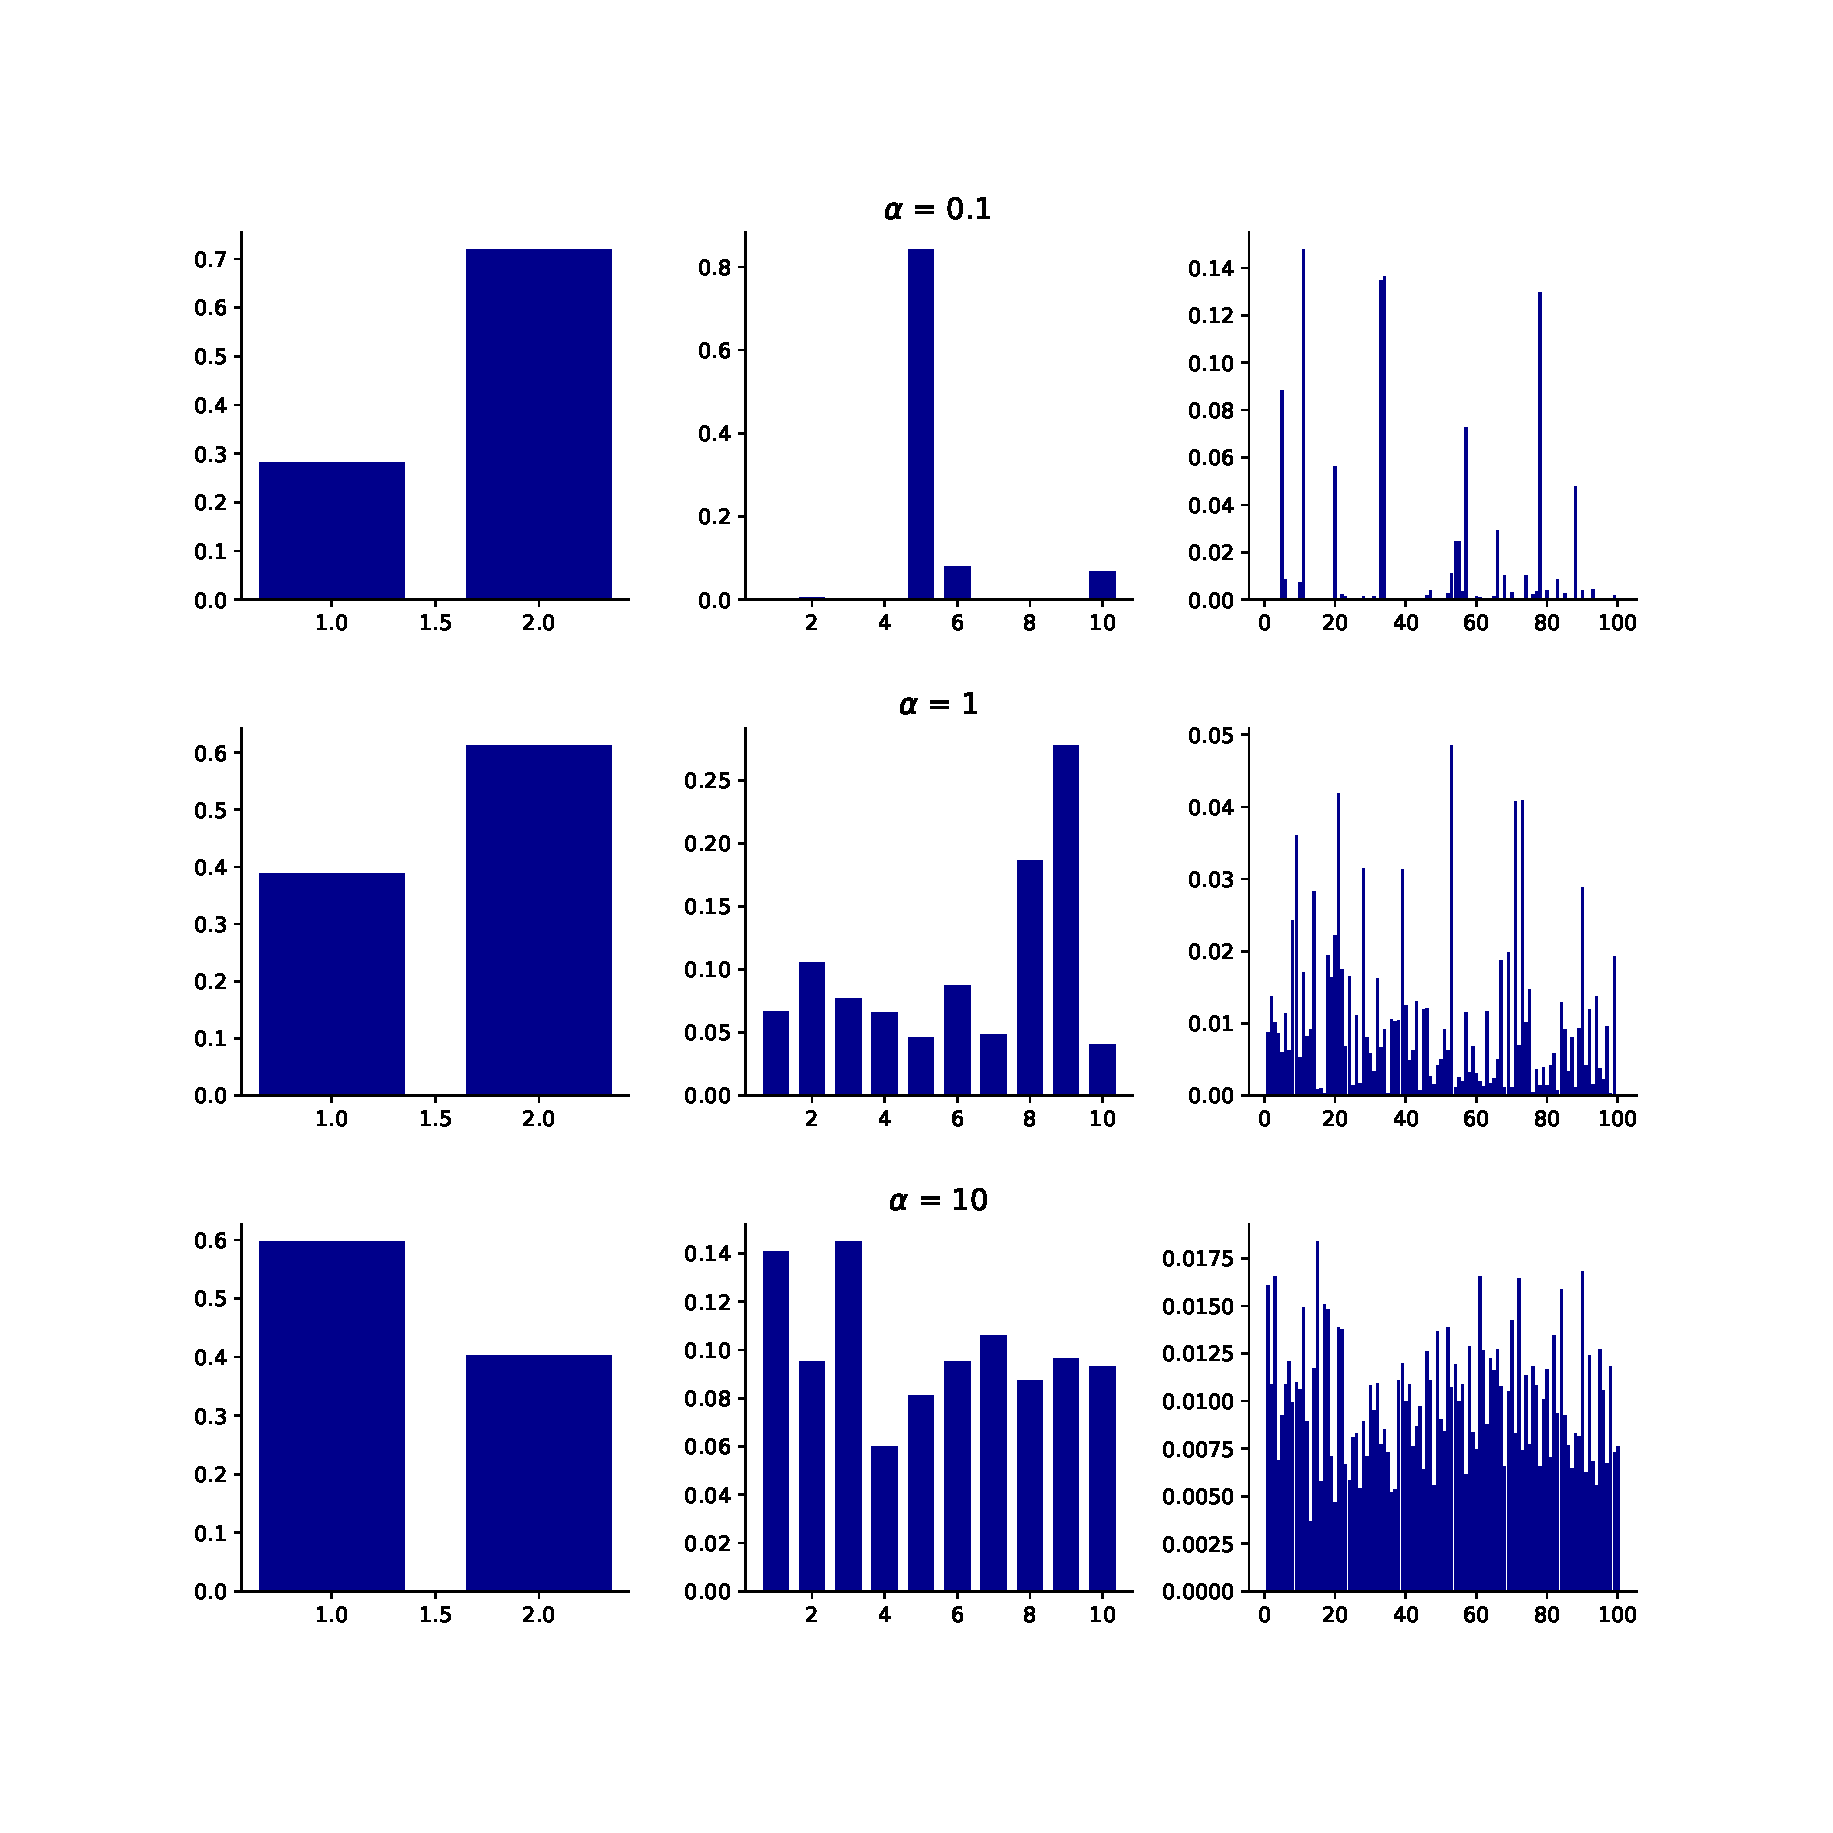
\includegraphics[width=\textwidth]{ch2/dirichlet_samples.eps}
    \caption{Muestra de una distribución Dirichlet simétrica para $\alpha \in \{0.1, 1, 10\}$ y $K\in\{2, 10, 100\}$.}
    \label{img:dirichlet_samples}
\end{figure}

\subsection{Dirichlet Process}
\label{sec:dp}

En un \textit{finite mixture model} tenemos $G(\phi) = \sum_{k=1}^{K} \pi_{k}\delta_{\phi_{k}}(\phi)$, luego si muestreamos a partir de $G$, siempre (con probabilidad uno) obtendrémos exactamente $K$ \textit{clusters}. Nos gustaría tener un modelo más flexible, que pueda generar un número variable de \textit{clusters}. La forma de hacer esto es remplazar la distribución discreta $G$ por una medida aleatoria de probabilidad. El Dirichlet Process, denotado $G\sim DP(\alpha, H)$, es una manera de hacer esto.\\

Un \textbf{Dirichlet Process} (DP) es una distribución sobre medidas de probabilidad $G: \Phi \rightarrow \mathbb{R}^{+}$, donde $G(\phi)\geq 0$ y $\int_{\Phi}G(\phi)d\phi=1$. Un DP se define implícitamente por cumplir 

\begin{align}
    (G(T_{1}), \ldots, G(T_{K})) \sim Dir(\alpha H(T_{1}), \ldots, \alpha H(T_{k}))
\end{align}

para cualquier partición finita $(T_{1}, \ldots, T_{k})$ de $\Phi$. En este caso, decimos que $G\sim DP(\alpha, H)$, donde $\alpha$ es llamado el \textbf{parámetro de concentración} y $H: \Phi \rightarrow \mathbb{R}^{+}$ es llamado la \textbf{medida base}.\\

Existen diferentes perspectivas que ayudan a entender la propiedad de \textit{clustering} de un Dirichlet Process. En la sección \ref{sec:sbp}. y \ref{sec:crp}. nos referimos a dos: el Stick Breaking Process y Chinese Restaurant Process (CRP).

\subsection{Stick Breaking Process}
\label{sec:sbp}

Ahora daremos una definición constructiva para el DP, conocida como \textit{stick breaking process}. Sea $\pi=\{\pi_{k}\}_{k=1}^{\infty}$ una secuencia infinita de mezcla de pesos derivadas a partir del siguiente proceso:
\begin{align}
    \beta_{k} & \sim Beta(1, \alpha)\\
    \pi_{k} & = \beta_{k}\prod_{l=1}^{k-1}(1-\beta_{l}) = \beta_{k}(1-\sum_{l=1}^{k-1}\pi_{l})
\end{align}

Esto se suele denotar como $\pi \sim GEM(\alpha)$, donde GEM representa Griffiths, Engen y McCloskey, ver Figura  \ref{img:stick_breaking} para una ilustración. 

\begin{figure}
    \centering
    \includegraphics[width=0.6\textwidth]{ch2/stick_breaking.png}
    \caption{Ilustración de \textit{stick breaking process}. Tenemos una barra de largo 1, la cual se rompe en un punto aleatorio $\beta_{1}$, el largo de la pieza que conservamos es llamada $\pi_{1}$, luego recursivamente rompemos la barra restante, así generando $\pi_{2}, \pi_{3}, \ldots$. Fuente: Figura 2.22 de \citep{sudderth2006graphical}.}
    \label{img:stick_breaking}
\end{figure}

Algunos ejemplos de este proceso son mostrados en la Figura \ref{img:dp_samples}. A mayor $\alpha$, menos varianza y mayor número de átomos, por el contrario, pequeños valores de $\alpha$ muestran una alta varianza y menor número de átomos, adicionalmente exhiben mayor varianza en el número de átomos.

\begin{figure}
    \centering
    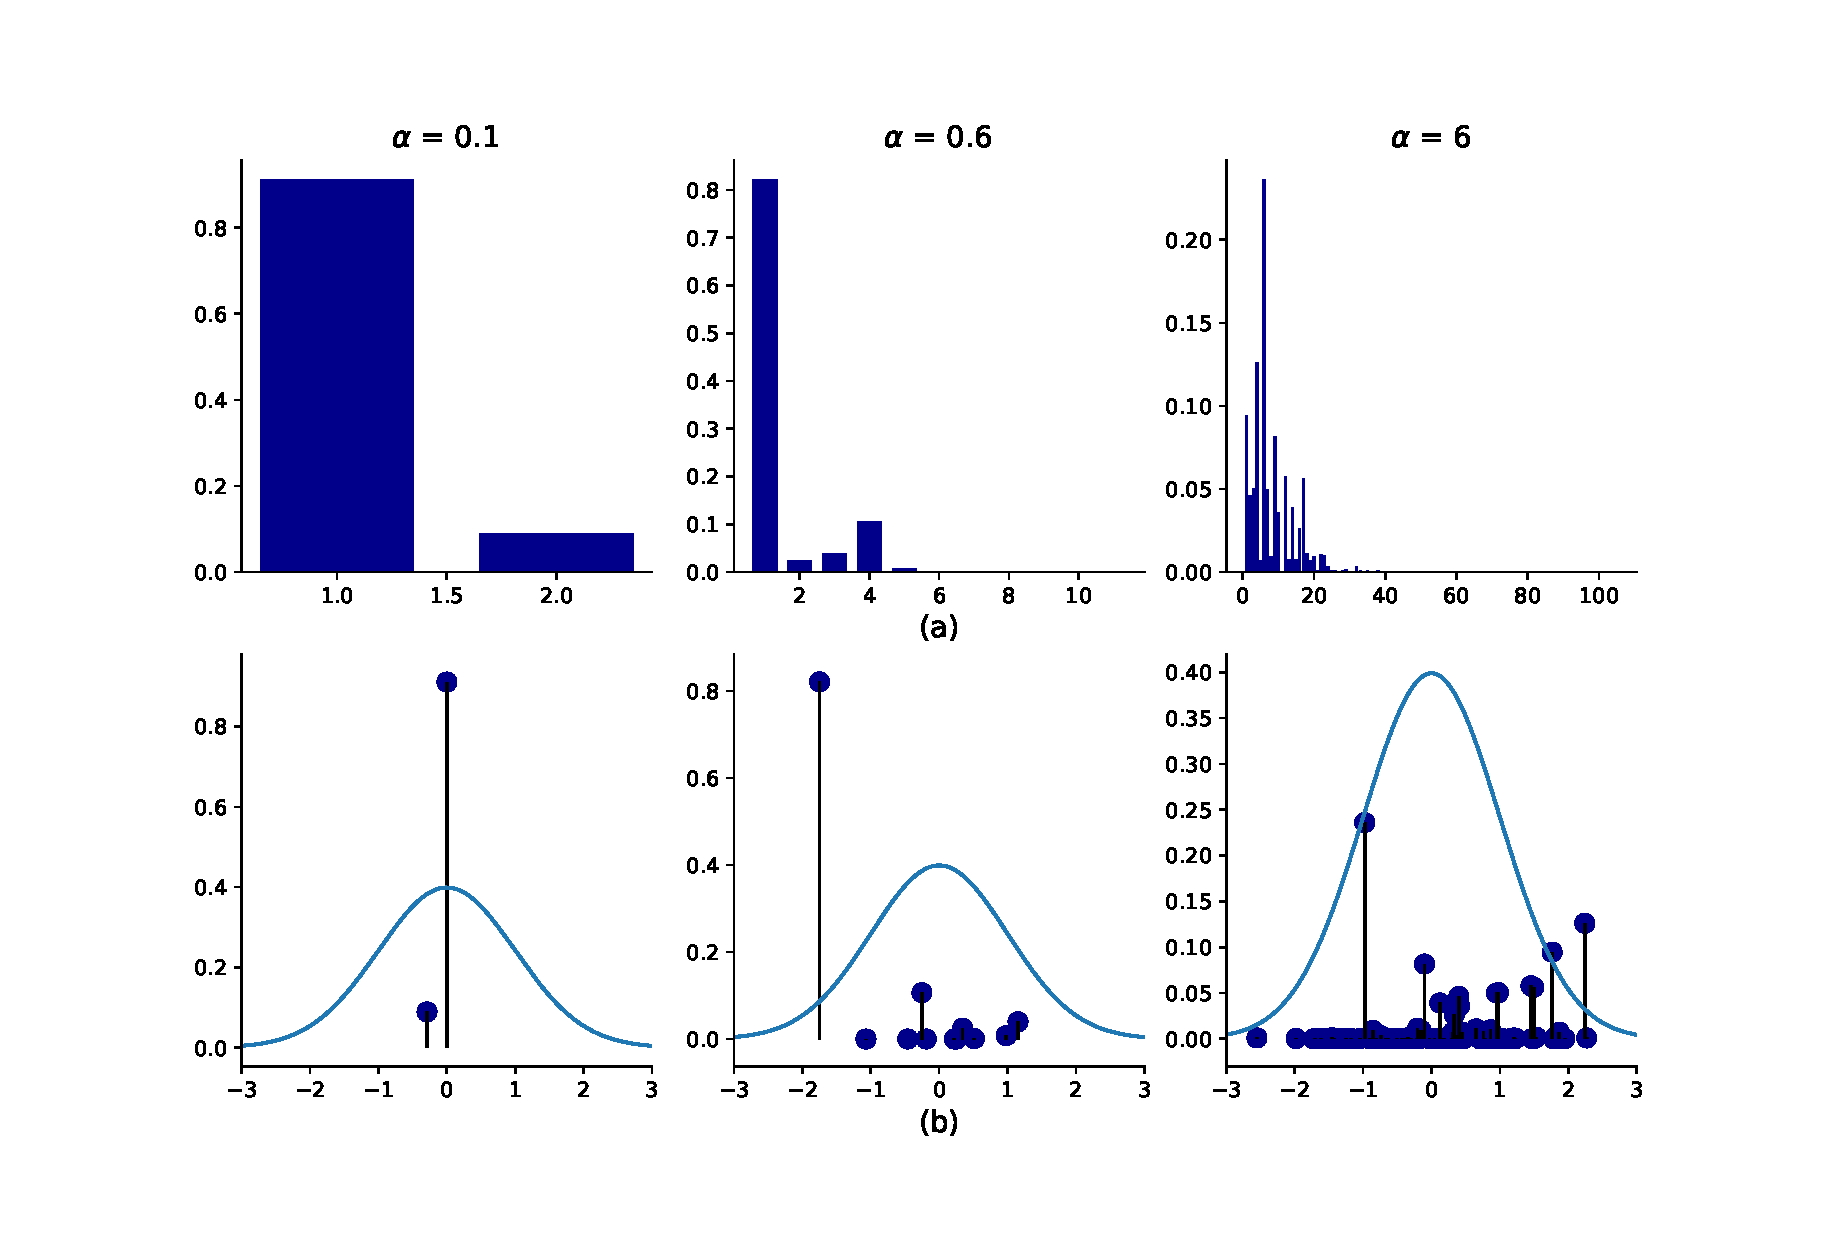
\includegraphics[width=\textwidth]{ch2/dp_samples.eps}
    \caption{(a) Muestra de una distribución GEM para diferentes parámetros de concentración $\alpha\in \{0.1, 0.6, 6\}$. (b) Medidas aleatorias generadas a partir de un Dirichlet Process con medida base normal $\mathcal{N}(0,1)$ para diferentes parámetros de concentración $\alpha\in \{0.1, 0.6, 6\}$}
    \label{img:dp_samples}
\end{figure}

Se puede demostrar que este proceso terminará con probabilidad uno, a pesar que el número de elementos que este genera incrementa con $\alpha$. Además, el tamaño del componente $\pi_{k}$ decrece en promedio. Ahora definamos 
\begin{align}
    G(\phi) = \sum_{k=1}^{\infty}\pi_{k}\delta_{\phi_{k}}(\phi)
\end{align}

donde $\pi \sim GEM(\alpha)$ y $\phi_{k} \sim H$. Entonces uno puede demostrar que $G \sim DP(\alpha, H)$. Como consecuencia de esta construcción, las muestras de un DP son \textbf{discretas con probabilidad uno}. En otras palabras, al ir muestreando $\bar{\phi_{i}}\sim G$ veremos valores repetidos, por lo que la mayoría de los datos vendrán de los $\phi_{k}$ con $\pi_{k}$ más largos. En la Figura \ref{img:dp_samples} muestra un par de medidas aleatorias generadas a partir de un DP con una medida base normal.\\


\subsection{Chinese Restaurant Process}
\label{sec:crp}

\todo[inline]{Describir Chinese Restaurant Process}

\section{Modelos de tópicos}

\todo[inline]{Motivar modelamiento de tópicos}
\todo[inline]{Motivar clustering sharing parameter y luego LDA-HDP}

% En este capitulo se describe en detalle dos modelos de tópicos probabilísticos,  Latent Dirichlet Allocation (LDA) y Hierarchical Dirichlet Process (HDP), siendo este último la generalización no parámetrica de LDA, donde el número de tópicos a descubrir no está acotado y se infiere a partir del corpus.\\

% Ambos modelos se consideran modelos de clustering que involucran multiples grupos de datos. Como los modelos de tópicos se suelen aplicar al dominio del texto a la colección de grupos se le llama corpus y a cada grupo se le llama documento, siendo un documento una colección palabras u observaciones. 

% Los modelos de tópicos trabajan bajo el asumpción de \textit{bag of words}, es decir, las palabras son intercambibles, por lo que podemos aplicar un modelo de clustering probabilístico a nivel documento, esto significa asumir que lo que las realizaciones independientes de un \textit{mixture model}

\subsection{Latent Dirichlet Allocation}\todoupdate{Mejorar estilo de redacción}

A continuación se describe el proceso generativo de Latent Dirichlet Allocation (LDA). Sean \textit{K} tópicos, $\phi_{1:K}$ distribuciones de probabilidad sobre un vocabulario fijo, dibujadas por una $Dir(\frac{\eta}{|V|}1_{|V|})$. Para cada documento $d$ del corpus $D$ se asume que es dibujado por el siguiente proceso generativo (ver representación gráfica del modelo en la Figura \ref{img:lda}):
\begin{enumerate}
    \item Dibujar una mezcla de tópicos $\pi_{d}\sim Dir(\frac{\alpha}{K}1_{K})$
    \item Para cada palabra:
    \begin{enumerate}
        \item Escoger un tópico $z_{d,n}\sim Mult(\pi_{d})$
        \item Escoger una palabra $w_{d,n}\sim Mult(\phi_{z_{d,n}})$
    \end{enumerate}
\end{enumerate}

\begin{figure}
  \centering
  \tikz{ %

    \node[latent, dashed] (alpha) {$\alpha$} ; %
    \node[latent, right=of alpha] (pi) {$\pi_{d}$} ; %
    \node[latent, right=of pi] (z) {$z_{d,n}$} ; %
    \node[obs, right=of z] (w) {$w_{d,n}$}   ; %
    \node[latent, right=of w] (phi) {$\phi_{k}$} ; %
    \node[latent, right=of phi, dashed] (eta) {$\eta$} ;%
    \plate[inner sep=0.25cm, xshift=-0.12cm, yshift=0.12cm] {plate1} {(z) (w)} {$N_{d}$}; %
    \plate[inner sep=0.25cm, xshift=-0.12cm, yshift=0.12cm] {plate2} {(pi) (plate1)} {$D$}; %
    \plate[inner sep=0.25cm, xshift=-0.12cm, yshift=0.12cm] {plate3} {(phi)} {$K$}; %
    \edge {alpha} {pi} ; %
    \edge {pi} {z} ; %
    \edge {z,phi} {w} ; %
    \edge {eta} {phi} ; %
  }
\caption{Representación gráfica de LDA: círculos denotan variables aleatorias, círculos abiertos denotan parámetros, círculos sombreados denotan variables observadas y los platos indican replicación.}
\label{img:lda}
\end{figure}

La probabilidad conjunta del modelo:
\begin{equation}
    p(\phi, \pi, z, w|\alpha, \eta)= \prod_{k=1}^{K}p(\phi_{k}|\eta)\prod_{d=1}^{D}p(\pi_{d}|\alpha)\prod_{n=1}^{N_{d}}p(z_{n,d}|\pi_{d})p(w_{d,n}|\phi_{1:K}, z_{d,n})
\end{equation}

La distribución a posterior:
\begin{equation}
    p(\phi, \pi, z|w, \alpha, \eta) = \frac{p(\phi, \pi, z, w|\alpha, \eta)}{p(w|\alpha, \eta)}
\end{equation}

La distribución posterior es computacionalmente intratable para inferencia exacta, debido a que para normalizar la distribución debemos marginalizar sobre todas las variables ocultas y escribir la constante de normalización en términos de los parámetros del modelo. Para poder computar la posterior es necesario utilizar algoritmos de inferencia aproximada, donde el enfoque habitual es Markov Chain Monte Carlo (MCMC), en \citep{griffiths2004finding} se propone un algoritmo basado en Gibbs Sampling para la inferencia. Los métodos basados en MCMC entregan una estimación empírica de la distribución posterior llamada (traza), es decir, representan la posterior a través de muestras que distribuyen como esta, luego para estimación puntual, como por ejemplo obtener el valor esperado de la posterior se utiliza integración de Monte Carlo para aproximar la esperanza, esto es promediar los valores de la traza.

Una representación equivalente en LDA sería generar cada palabra de un documento $d$ a partir de una multinomial sobre un tópico dibujado por una distribución $G_{d}$, formalmente, $w_{d,n}\sim Mult(\phi_{d,n})$, donde $\phi_{d,n} \sim G_{d}$ con $\phi_{d,n} \in \{\phi_{k}\}_{k=1}^{K}$, y $G_{d}(\phi)=\sum_{k=1}^{K}\pi_{d, k}\delta_{\phi_{k}}(\phi)$, donde $\delta_{\phi_{k}}(\phi) = \begin{cases}
    1 & \text{si $\phi_{k}=\phi$}  \\
    0 & \text{si no}
  \end{cases}$.\\\\

\subsection{Hierarchical Dirichlet Process}\todoupdate{Mejorar estilo de redacción}

Hierarchical Dirichlet Process (HDP) es una colección de DP que comparten una distribución base $G_{0}$, la cual además es dibujada a partir de un DP (ver representación gráfica del modelo en la Figura \ref{img:hdp}). Matemáticamente, a nivel corpus se tiene que la distribución base $H \sim Dir(\frac{1}{|V|}1_{|V|})$ y $G_{0} \sim DP(\gamma, H)$, luego, para cada documento $d$ del corpus $D$ se asume que es dibujado por el siguiente proceso generativo:
\begin{enumerate}
    \item Dibujar un DP $G_{d} \sim DP(\alpha_{0}, G_{0})$
    \item Para cada palabra:
    \begin{enumerate}
        \item Dibujar un tópico $\phi_{d,n}\sim G_{d}$
        \item Escoger una palabra $w_{d,n} \sim Mult(\phi_{d,n})$
    \end{enumerate}
\end{enumerate}

\begin{figure}
  \centering
  \tikz{ %
    \node[latent, dashed] (H) {$H$} ; %
    \node[latent, right=of H] (G0) {$G_{0}$} ; %
    \node[latent, above= of G0, dashed] (gamma) {$\gamma$} ; %
    \node[latent, right=of G0] (Gd) {$G_{d}$} ; %
    \node[latent, above= of Gd, dashed] (alpha0) {$\alpha_{0}$} ; %
    \node[latent, right= of Gd] (phi) {$\phi_{d,n}$} ; %
    \node[obs, right=of phi] (w) {$w_{d,n}$}   ; %
    \plate[inner sep=0.25cm, xshift=-0.12cm, yshift=0.12cm] {plate1} {(phi) (w)} {$N_{d}$}; %
    \plate[inner sep=0.25cm, xshift=-0.12cm, yshift=0.12cm] {plate2} {(Gd) (plate1)} {$D$}; %
    \edge {H, gamma} {G0} ; %
    \edge {G0, alpha0} {Gd} ; %
    \edge {Gd} {phi} ; %
    \edge {phi} {w} ; %
  }
\caption{Representación gráfica de HDP: círculos denotan variables aleatorias, círculos abiertos denotan parámetros, círculos sombreados denotan variables observadas y los platos indican replicación.}
\label{img:hdp}
\end{figure}

La discretitud a nivel corpus de $G_{0}$ asegura que todos los documentos comparten el mismo conjunto de tópicos (\textit{mixture components}). A nivel documento $G_{d}$ hereda los tópicos de $G_{0}$, pero los pesos de cada tópico (\textit{mixture proportions}) es específica del documento.\\

Aplicando \textit{stick breaking construction} se tiene que para el DP dibujado a nivel corpus la siguiente representación:

\begin{align}
    \beta_{k}^{'} \sim Beta(1, \gamma) \\
    \beta_{k} = \beta_{k}^{'}\prod_{l=1}^{k-1}(1-\beta_{l}^{'})\\
    \phi_{k} \sim H  \\
    G_{0}(\phi)=\sum_{k=1}^{\infty}\beta_{k}\delta_{\phi_{k}}(\phi)
\end{align}

Así, $G_{0}$ es discreto y tiene soporte en los átomos $\phi = \{\phi\}_{k=1}^{\infty}$ con pesos $\beta=\{\beta_{k}\}_{k=1}^{\infty}$, siendo la distribución de $\beta$ escrita como $\beta \sim GEM(\gamma)$. La construcción a nivel documento de $G_{d}$ es:

\begin{align}
    \pi_{d,k}^{'}\sim Beta\big(\alpha_{0}\beta_{k}, \alpha_{0}\big(1-\sum_{l=1}^{k}\beta_{l}\big)\big)\\
    \pi_{d,k} = \pi_{d,k}^{'}\prod_{l=1}^{k-1}(1-\pi_{d,l}^{'})\\
    G_{d}(\phi)=\sum_{k=1}^{\infty}\pi_{d,k}\delta_{\phi_{k}}(\phi)
\end{align}

Donde $\phi = \{\phi_{k}\}_{k=1}^{\infty}$ son los mismos átomos de $G_{0}$. En la Figura \ref{img:hdp_sbc} se muestra la representación gráfica de esta construcción.

%stick breaking
\begin{figure}
  \centering
  \tikz{ %
    \node[latent] (beta) {$\beta$} ; %
    \node[latent, above= of beta, dashed] (gamma) {$\gamma$} ; %
    \node[latent, right=of beta] (pi) {$\pi_{d}$} ; %
    \node[latent, above= of pi, dashed] (alpha0) {$\alpha_{0}$} ; %
    \node[latent, right= of pi] (z) {$z_{d,n}$} ; %
    \node[obs, right=of z] (w) {$w_{d,n}$}   ; %
    \node[latent, right=of w] (phi) {$\phi$} ; %
    \node[latent, above=of phi, dashed] (H) {$H$} ; %
    \plate[inner sep=0.25cm, xshift=-0.12cm, yshift=0.12cm] {plate1} {(z) (w)} {$N_{d}$}; %
    \plate[inner sep=0.25cm, xshift=-0.12cm, yshift=0.12cm] {plate2} {(pi) (plate1)} {$D$}; %
    \plate[inner sep=0.25cm, xshift=-0.12cm, yshift=0.12cm] {plate3} {(phi)} {$K (\infty)$}; %
    \edge {gamma} {beta} ; %
    \edge {beta, alpha0} {pi} ; %
    \edge {pi} {z} ; %
    \edge {z, phi} {w} ; %
    \edge {H} {phi} ; %
  }
\caption{Representación gráfica de la construcción stick-breaking de HDP: circulos denotan variables aleatorias, circulos abiertos denotan parámetros, círculos sombreados denotan variables observadas y los platos indican replicación.}
\label{img:hdp_sbc}
\end{figure}

Al igual que LDA la distribución posterior es intratable, por lo que en \citep{teh2005sharing} se marginaliza $G_{0}$ y $G_{d}$'s afuera, obteniéndose así un nuevo proceso generativo denominado \textit{Chinese restaurant franchise process} (CRF), esta representación permite construir algoritmos eficientes basados en Gibbs Sampling, como en la implementación utilizada disponible en \citep{HDP}.

\subsubsection{LDA versus HDP}\todoupdate{Mejorar estilo de redacción}
HDP es un modelo no paramétrico similar en estructura a LDA, la principal desventaja de LDA frente a HDP es que LDA requiere escoger el número de tópicos $K$ por adelantado, por otro lado, en HDP el número de tópicos no está acotado y es inferido a partir de los datos. En un enfoque tradicional, se requiere de entrenar múltiples veces LDA para diferentes valores de $K$ y se escoge el que tiene mejor la configuración con mejor desempeño en un conjunto de validación, por lo que LDA termina siendo computacionalmente más costoso que HDP, además este enfoque se vuelve impracticable cuando el conjunto de datos es grande. En el aspecto cualitativo ambos modelos entregan tópicos igual de consistentes, en cuanto a métricas de desempeño como $\textit{perplexity}$ HDP suele tener mejor desempeño \citep{teh2005sharing}.

\subsection{Interpretación de tópicos}\todoupdate{Mejorar estilo de redacción}
Los modelos de tópicos se caracterizan por tener un alto poder interpretativo, esto se debe a que la distribución de probabilidad de cada tópico sobre el vocabulario nos da una idea del tema al que pertenece, por otro lado la mezcla de tópicos de cada documento muestra que tan importante es cada tópico en la generación de estos, como también dentro del corpus. En este sentido, las visualizaciones nos ayudan a interpretar mejor los resultados de los modelos de tópicos, respondiendo a las siguientes preguntas, ¿Cuál es el significado de cada tópico?¿Cuán predonimnante es cada tópico?¿Cómo se relacionan los tópicos entre sí?\\

En \citep{sievert2014ldavis} desarrollaron una herramienta de visualización web para responder a estas preguntas. Para responder la pregunta 1 se incorpora un gráfico de barras que muestra las palabras más relevantes del tópico seleccionado dado un parámetro $\lambda \in [0,1]$. A través de una visualización espacial responde la pregunta 2 y 3. La visualización espacial consiste en aplicar técnicas de reducción de dimensionalidad como TSNE \citep{maaten2008visualizing} o PCA \citep{wold1987principal} (en este caso se utilizó TSNE) a la matriz de distancia entre tópicos, usando Jensen-Shannon divergence \citep{endres2003new} como médida de distancia. Una vez cada tópico es mapeado a un punto en un espacio de dos dimensiones se dibuja un círculo con centro en este punto y con radio proporcional a la cantidad de tokens generados por el tópico.\\

Para interpretar un tópico, uno típicamente examina una lista ordenada de los palabras más probables en el tópico, usando ya sea desde cinco a treinta términos. Un problema frecuente que se presenta en este caso es que los términos que son comunes al corpus frecuentemente aparecen en el top de las palabras más probables de un tópico, haciendo difícil discernir el significado de estos.
Para esto en \citep{sievert2014ldavis} se define una métrica denominada \textit{relevance}, la cual define la relevancia de una palabra no solo por su probabilidad dentro del tópico sino también por su exclusivad dentro del corpus. La \textit{relevance} de una palabra $w$ en el tópico $k$ dado $\lambda$ está dada a través de la siguiente expresión:

\begin{align}
    r(w,k|\lambda) = \lambda log (\phi_{kw})+ (1-\lambda)\lambda log\bigg(\frac{\phi_{kw}}{p_{w}}\bigg)
\end{align}

, donde $\lambda$ determina el peso que se le da a la probabilidad de la palabra $w$ dentro del tópico $k$ ($\phi_{kw}$) relativo a su \textit{lift}, el cual se define por el ratio entre la probabilidad de la palabra dentro del tópico y su probabilidad marginal a lo largo del corpus ($p_w$). Fijando $\lambda=1$ se obtiene el ranking de términos decrecientes en orden de su probabilidad dentro del tópico, y fijando $\lambda=0$ el ranking se basa solo en el \textit{lift}.

\section{Modelamiento de la evolución de los tópicos en el tiempo}

\todo[inline]{Motivar}

Nuestro objetivo es modelar la evolución en el tiempo de los tópicos, para esto el corpus es divido en $T$ épocas, en cada época se entrena un modelo de tópicos estático, obteniéndose así $T$ conjuntos de tópicos $\phi=\{\phi_{1}, \ldots, \phi_{T}\}$, donde $\phi_{t}=\{\phi_{t,1}, \ldots, \phi_{t,K_{t}}\}$ es el conjunto de tópicos que describen la época $t$, y $K_{t}$ el número de tópicos inferido en esa época.

\subsection{Gráfo de similitud temporal}\todoupdate{Mejorar estilo de redacción}

Para relacionar los tópicos de una época necesitamos una medida de similitud $\rho \in [0,1]$, con esta médida de similitud se puede construir un gráfo, donde los nodos son los tópicos de una época y los arcos relacionan tópicos de una época con la siguiente, siendo el peso del arco la similitud entre los tópicos. Una vez construido el grafo se eliminan las conexiones débiles en base a un umbral $\zeta \in [0,1]$ a definir, reteniendo solo aquellas conexiones entre tópicos suficientemente similares entre épocas adyacentes, matemáticamente podamos el arco entre los tópicos $\phi_{t,i}$ y $\phi_{t+1,j}$ si $\rho(\phi_{t,i}, \phi_{t+1,j})\leq \zeta$. Una ilustración conceptual del grafo de similitud es mostrado en la Figura \ref{img:graph}, este muestra tres épocas consecutivas.

\begin{figure}
    \centering
    \includegraphics[width=0.8\textwidth]{ch2/similarity_graph.png}
    \caption{Ilustración conceptual del grafo de similitud que modela la dinámica de los tópicos en el tiempo. Un nodo corresponde a un tópico en una época específica; el ancho de los arcos es proporcional a la similitud entre los tópicos, arcos ausentes fueron eliminados por presentar una similitud menor a un umbral.}
    \label{img:graph}
\end{figure}

Está metodología permite fácilmente detectar desaparición de un tópico, nacimiento de un nuevo tópico, como también dividir o fusionar diferentes tópicos, a continuación se define en detalle cada uno de estos dinamismos:

\begin{itemize}
    \item \textbf{Nacimiento de un tópico:} Si un tópico no tiene ningún arco entrante, por ejemplo, en la Figura \ref{img:graph} el tópico $\phi_{j+2}$ en $t$.
    \item \textbf{Muerte de un tópico:} Si un tópico no tiene ningún arco saliente, por ejemplo, en la Figura \ref{img:graph} el tópico $\phi_{j}$ en $t$.
    \item \textbf{Evolución de un tópico:} Cuando un tópico tiene exactamente un arco de entrada y salida, por ejemplo, en la Figura \ref{img:graph} entre las épocas $t$ y $t+1$ se tiene que el tópico $\phi_{j+2}$ evoluciona del tópico $\phi_{k+1}$.
    \item \textbf{División de un tópico:} Si un tópico tiene más de un arco saliente, por ejemplo, en la Figura \ref{img:graph} el tópico $\phi_{i}$ de $t-1$ se divide en $t+1$ en los tópicos $\phi_{j}$ y $\phi_{j+1}$.
    \item \textbf{Fusión de un tópico:} Cuando un tópico tiene más de un arco entrante, este tipo de tópicos también pueden ser entendidos como un nuevo tópico, por ejemplo, en la Figura \ref{img:graph} los tópicos $\phi_{i}$ y $\phi_{i+1}$ de $t-1$ forman al tópico $\phi_{j+1}$ en $t$.
\end{itemize}

Un aspecto relevante de esta metodología es definir el úmbral de corte, el cual no es fácilmente interpretable, además el úmbral depende de la médida de similitud escogida, dificultando así la comparación entre médidas de similitud. En \cite{beykikhoshk2018discovering} proponen una alternativa más interpretable para definir el úmbral, para esto estiman la función de distribución acumulada (cdf) del grafo inicial, donde todos los nodos de una época están conectados con todos los nodos de la época adyacente, sea $F_{p}$ la cdf sobre las similitudes del grafo inicial, luego sea $\zeta \in [0,1]$ el punto operante de la cdf, luego eliminamos el arco entre los tópicos $\phi_{t,i}$ y $\phi_{t+1,j}$ si $\rho(\phi_{t,i}, \phi_{t+1,j})\leq F_{p}^{-1}(\zeta)$, donde  $F_{p}^{-1}(\zeta)$ es el cuantil $\zeta$ de $F_{p}$.

\subsection{Medidas de similitud}\todoupdate{Mejorar estilo de redacción}

Los tópicos son distribuciones de probabilidad sobre un vocabulario fijos de términos. La gran mayoría de medidas de similitud comparan vectores con el mismo dominio y dimensión, esto significa que los tópicos de épocas adyacentes deben compartir el mismo vocabulario, matemáticamente, sea $\phi_{t, i}$ un tópico de la época $t$ y $V_{t}$ su vocabulario, sea  $\phi_{t+1, j}$ un tópico de la época $t+1$ y $V_{t+1}$ su vocabulario, lo más probables es que existan palabras en $V_{t}$ que no existan en $V_{t+1}$ y viceversa, para poder comparar tópicos en estas épocas adyacentes se debe construir el vocabulario $V_{t+1}^{'}=V_{t}\cup V_{t+1}$, luego se aplica $padding$ a los vectores $\phi_{t, i}$ y $\phi_{t+1, j}$, es decir, se rellenan con ceros las posiciones de palabras que no están en el vocabulario de su dominio.\\

La gran desventaja del enfoque anterior es que no captura similitud entre palabras, es decir, dos palabras diferentes que pueden llegar a ser sinónimos ocuparan una posición diferente dentro del vector, siendo no robusta a cuando una palabra esta presente en la época $t$ y no en $t-1$ por lo que no hay forma de compararla por ejemplo con la palabra de $t-1$ más símil, por lo que se compara la palabra consigo misma, donde en $t$ tiene un peso distinto de cero y en $t-1$ un peso nulo. El peor caso sería considerar los vocabularios $V_{t}$ y $V_{t+1}$, donde $V_{t}\cap V_{t+1} =  \emptyset$, a pesar de que cada palabra en $V_{t}$ tiene un sinónimo en $V_{t+1}$ la similitud entre tópicos entre las épocas $t$ y $t+1$ sería cero.\\

Para lidiar con el problema anterior en \citep{kusner2015word} se propone una medida de distancia llamada Word Mover's Distance (WMD) para comparar dos documento bajo una representación \textit{bag of words}, donde $i$ y $j$ son los documentos, $V_{i}$ y $V_{j}$ los vocabularios, y el peso asociado a cada palabra de un documento  es igual a la frecuencia normalizada. Generalizar al caso de tópicos es bastante sencillo, puesto a que estos se construyen bajo una representación bag of words, por ejemplo, para comparar el tópico $i$ de la época $t$ con el tópico $j$ de la época $t+1$, se usan los pesos $\phi_{t,i}$ y $\phi_{t+1,j}$ sobre el vocabulario $V_{t}$ y $V_{t+1}$ respectivamente. WMD calcula el costo mínimo de transformar un documento en otro, en esto caso particular sería el costo mínimo de llevar un tópico a otro, para esto se resuelve el problema de transporte, donde los flujos son los pesos $\phi_{t,i}$ y $\phi_{t+1,j}$ y la matriz de costos es una matriz de distancia euclidiana entre los \textit{word embedding} (\cite{mikolov2013distributed}) de todas las palabras de $V_{t}$ con $V_{t+1}$. Para resolver este problema se utilizó la implementación de \citep{PyEMD}. En la Figura \ref{img:wmd_obama} se ilustra el espacio en el que viven las palabras de dos tópicos.

\begin{figure}
    \centering
\includegraphics[width=1\textwidth]{ch2/wmd-obama.png}
    \caption{Espacio vectorial de los \textit{word embeddings} de las palabras de dos tópicos con un vocabulario de tamaño 4.}
    \label{img:wmd_obama}
\end{figure}\todoref{Citar}

Matemáticamente, la WMD entre el tópico $i$ de la época $t$ y el tópico $j$ de la época $t+1$ viene dado por $WMD(\phi_{i,t}, \phi_{j,t+1})$:

\begin{align}
\underset{T}{\text{minimize}}&\sum_{u \in V_{t}}\sum_{v \in V_{t+1}} c_{u,v}T_{u,v} \\ 
\textrm{s.t.}\qquad &\sum_{v \in V_{t+1}}T_{u,v}= \phi_{i,t,u} \;, u \in V_{t}\\ 
& \sum_{u \in V_{t}}T_{u,v}= \phi_{j,t+1,v} \;, v\in V_{t+1}\\
& T_{u,v} \geq 0,\; u \in V_{t} \;, v \in V_{t+1}\\ \nonumber
\end{align}

Donde $T_{u,v}$ es el flujo que va de la palabra $u$ del tópico $i$ de la época $t$ a la palabra $v$ del tópico $j$ de la época $t+1$, $\phi_{i,t,u}$, es la probabilidad de la palabra $u$ en el tópico $i$ de la época $t$, $c_{u,v}$ es el costo de mover una unidad de flujo por el arco $(u,v)$, el costo entre palabras se mide como la distancia euclidiana entre los \textit{word embedding} de dichas palabras. La primera restricción indica que el flujo que se mueve de una palabra $u$ del tópico $i$ a todas las palabras del tópico $j$ debe sumar su peso ($\phi_{i,t,u}$), la segunda restricción significa que el flujo que se mueve de una palabra $v$ del tópico $j$ a todas las palabras del tópico $i$ debe sumar su peso ($\phi_{j,t+1,v}$). Esta médida de distancia se puede fácilmente transformar en una médida de similitud $\rho(\phi_{i,t}, \phi_{j,t+1}) = \frac{1}{1+WMD(\phi_{i,t}, \phi_{j,t+1})}$, notar que si la WMD es 0 la similitud es 1 y si es $\infty$ la similitud es 0. \\

WMD es una medida de distancia intensiva en recursos computacionales, para entender mejor esto utilizaremos la representación poliedral del problema, sea $N$ el tamaño del vocabulario entre dos épocas adyacentes, luego la región factible del problema anterior se puede representar como $\{x| Ax=b, x\geq 0\}$, con $A\in \mathbb{R}^{2N\times N^{2}}$ la matriz de costos, $b\in \mathbb{R}^{2N}$ el flujo disponible y $x\in \mathbb{R}^{N}$ el flujo a enviar por cada uno de los arcos, la complejidad del mejor tiempo promedio de resolver este problema de optimización escala $\mathcal{O}(N^{2}log N)$ \citep{pele2009fast}, por lo que si se reduce el vocabulario a un décimo esto trae una reducción de al menos unas 200 veces (en el peor caso promedio). Los tópicos siguen una distribución de ley de potencia sobre el vocabulario, donde una fracción de las palabras concentran la mayor parte de la masa de la distribución. Además, en la práctica la interpretación de los tópicos se basa en los top $T$ palabras más probables (o relevantes) con $T \in [5, 30]$, entonces, podemos aprovechar esta estructura para efectos de computar la WMD de un forma más eficiente, por ejemplo, utilizando solo las palabras que capturan un 95\% de la distribución acumulada del tópico.

\todosec[inline]{Resumen Método propuesto}

\todosec[inline]{Métricas}

\todosec[inline]{Procesamiento}

\chapter{Experimento}
\todo[inline]{Motivación}
\todo[inline]{Describir organización del contenido}

\todosec[inline]{Diseño del experimento}

\section{Datos}\todosec{Descripción del dataset: mejorar estilo y añadir ejemplos}

Para este experimento se cuenta con las fuentes de datos de la Asociación de Aseguradores de Chile (AACH), corresponde a los relatos que las víctimas del robo de sus vehículos dan a las aseguradoras, lo cual corresponde a 49.015 relatos entre el 2011 y 2016.\\

% descripción detallada del conjunto de datos
% gráficos del Informe_1_fondef?
% hablar del nivel de granularidad, justificar en base facilidad de análisis de resultados, interpretación, largo del grafo, combinatoria, etc

Para el uso de WMD es necesario contar con \textit{words embeddings}, para esto se utilizaron los \textit{embeddings} de \citep{fastextSBWC}, estos \textit{embeddings} fueron obtenidos utilizando el algoritmo FastText \citep{bojanowski2017enriching} sobre el corpus Spanish Billion Word Corpus (SBWC) \citep{cardellinoSBWCE}. FasText en comparación a otros enfoques para extraer \textit{embeddings} representa los \textit{tokens} a través de n-gramas de caracteres, de esta manera se pueden obtener \textit{embeddings} de \textit{tokens} no vistos durante el entrenamiento a partir de los \textit{embeddings} de los caracteres que lo componen.

\section{Procesamiento}\todoredo{Rehacer}

En minería de texto con el objetivo de extraer el core de palabras del corpus se recurre métodos para reducir el vocabulario, la reducción del vocabulario mejora la significancia estadística de los modelos, puesto que se obtiene un mejor balance entre cantidad de parámetros y cantidad de observaciones, por otro lado puede verse fácilitada la interpretación de los tópicos al remover palabras que aportan poca información.\todo{Mover a marco teórico} \\

El paso cero en el procesamiento de textos es tokenizar, la tokenización es una operación sobre una cadena de carácteres (\textit{string}) que consiste en dividir el \textit{string} en un conjunto de términos, en este caso la división se hizo por el carácter espacio, como resultado de esto se obtiene una lista de elementos, a cada elemento de esta lista se le denomina \textit{token} que en términos simples puede considerarse como una palabra para el ejemplo mencionado\todo{Mover a marco teórico}. \\

Luego, en el primer nivel de procesamiento no interesa hacer distinción entre mayúsculas o minúsculas\footnote{En análisis de sentimiento puede ser interesante ya que las personas suelen expresar mensajes de enfado con letras capitales, por lo que las letras capitales añaden información al análisis.}, por ende, los carácteres de cada token son llevados a minúscula, también se eliminaron carácteres y tokens que no aportan información, como símbolos de puntuación, correos electrónicos y tokens que contienen números. En la figura \ref{img:cum_dist1} se observa la distribución acumulada de los tokens del corpus a este nivel de procesamiento, adicionalmente se tiene que el 50\% de los \textit{tokens} del vocabulario ocurren una sola vez, el 80\% tiene una ocurrencia menor o igual a 5 y el 95\% de la distribución acumulada puede ser explicada con 4199 \textit{tokens} (9\%) del vocabulario, se concluye que la distribución es sumamente pesada y es necesario recurrir a métodos adicionales para su reducción. \todo{Mover a marco teórico}\\

\begin{figure}
    \centering
    \includegraphics[width=0.8\textwidth]{ch3/cum_dist_1.png}
    \caption{Frecuencia acumulada de los tokens únicos aplicando hasta el primer nivel de procesamiento. El eje horizontal es el acumulado de tokens únicos en orden decreciente de ocurrencia. Los puntos corresponden a los cuantiles 60\%, 80\%, 90\%, 95\% y 99\%.}
    \label{img:cum_dist1}
\end{figure}\todoredo{Rehacer}

En el segundo nivel de procesamiento se eliminaron las \texit{stopwords}, palabras que aportan poca información, como artículos, preposiciones y conectores, para esto se utilizó la lista de \textit{stopwords} disponible en el paquete NLTK de Python \citep{bird2009natural} la cual cuenta con 313 palabras. Además, esta lista de \textit{stopwords} se alimentó con \textit{stopwords} contextuales, palabras específicas del corpus que aportan poca información, para esto se hizó un etiquetado de las 1000 palabras más frecuentes del corpus incorporando 417 nuevas palabras, algunos ejemplos son palabras que hacen referencia a vehículo y robo, puesto que todos los documentos corresponden a robos de vehículos.\todo{Mover a marco teórico}\\

El tercer nivel de procesamiento consiste en normalizar los tokens para reducir aún más el vocabulario, como métodos de normalización los más utilizados son \textit{stemming}  y lematización. \textit{Stemming} es el proceso de llevar una palabra a su raíz (\textit{stem}), en la práctica \textit{stemming} consiste en aplicar un algoritmo basado en ciertas reglas gramáticales para extraer sufijos \citep{porter1980algorithm}, como desventaja es que stemming no tiene en cuenta el contexto de la palabra por lo que la raíz obtenida puede no corresponder a la raíz verdadera de la palabra, además, para el caso de modelamiento de tópicos los tópicos se vuelve más difícil de interpretar, ya que palabras con significado completamente distinto terminan con la misma raíz o bien la raíz encontrada no tiene un significado claro. Por otro lado, lematización es el proceso de agrupar juntas las formas flexionadas de una palabra para que puedan analizarse como un elemento, identificado como lema, su diferencia principal con \textit{stemming} es que opera con conocimiento del contexto de la palabra para discriminar entre palabras que tienen significado diferente dependiendo del \textit{part of speech tagging} (POST) y de una tabla de búsqueda (\textit{lookup table}). Como método de normalización se decidió utilizar lematización en vez de \texit{stemming} debido a que tiene menos impacto en la interpretación de los tópicos, sin embargo es una operación más intensiva debido a que \texit{stemming} es un algoritmo basado en reglas simples mientras que en lematización se suele usar redes neuronales recurrentes (RNNs) para el POST y una vez determinadas las etiquetas gramaticales de las palabras en un documento se utiliza una \textit{lookup table} para encontrar el lema correspondiente. La implementación de lematización utilizada es la implementación de lematización en español del paquete spaCy de Python \citep{spacy2}.\todo{Mover a marco teórico}\\

El cuarto y último nivel de procesamiento corresponde a eliminar tokens con baja frecuencia, puesto que el modelo no será capaz de levantar patrones en tokens que aparecen una única vez o con una ocurrencia poco significativa, luego, como el corpus está particionado en épocas, se eliminaron aquellos tokens que aparecen en menos de 5 documentos dentro de una época.\todo{Mover a marco teórico}

\begin{figure}
    \centering
    \includegraphics[width=0.8\textwidth]{ch3/cum_dist_2.png}
    \caption{Frecuencia acumulada de los tokens únicos aplicando hasta el cuarto nivel de procesamiento. El eje horizontal es el acumulado de tokens únicos en orden decreciente de ocurrencia. Los puntos corresponden a los cuantiles 60\%, 80\%, 90\%, 95\% y 99\%.}
    \label{img:cum_dist2}
\end{figure}\todoredo{Rehacer}

En la figura \ref{img:cum_dist2} se presenta la distribución acumulada del vocabulario hasta el cuarto nivel de procesamiento, en donde se observa que la cola de distribución es bastante menos pesada que bajo el primer nivel de procesamiento, además, como se observa en la tabla \ref{table:processing_stats} el tamaño del vocabulario se redujo a menos de un décimo del vocabulario obtenido bajo el primer nivel de procesamiento y es menos de un décimo del tamaño del corpus, por lo que bajo este nivel de procesamiento es posible desarrollar modelos con mayor fuerza estadística.\todoredo{Rehacer}

\begin{table}[H]
    \begin{tabular}{|c|r|r|r|}
        \hline
        procesamiento & \multicolumn{1}{c|}{documentos} & \multicolumn{1}{c|}{vocabulario} & \multicolumn{1}{c|}{tokens} \\ \hline
        raw          & 49.015                           & 79.327                            & 2.030.980                     \\ \hline
        ch    & 49.011                           & 46.708                            & 1.947.235                     \\ \hline
        ch+s+l+f      & 47.993                           & 4.106                             & 508.987                      \\ \hline
        \end{tabular}
    \caption{Estadísticas del corpus bajo distintos niveles de procesamientos, \textbf{raw}: sin procesamiento, \textbf{ch}: eliminación de símbolos de puntuación, correos electrónicos y tokens con números, \textbf{ch+s+l+f}: además incluye eliminación de stopwords (s), lemmatización (l) y eliminación de tokens con baja ocurrencia (f).}
    \label{table:processing_stats}
\end{table}\todoredo{Rehacer}

En la tabla \ref{table:innovation_rate} se muestra el detalle del vocabulario para cada una de las épocas tras procesar el corpus, de aquí se extrae que en promedio un 21.28\% del vocabulario se olvida de una época a otra y un 28.19\% es nuevo, es otras palabras, en promedio alrededor de un 50\% del vocabulario no es común entre tópicos de épocas adyacentes, esto justifica la necesidad de utilizar médidas de similitud que capturen la similitud entre palabras de épocas adyacentes ante la renovación que sufre el vocabulario en el tiempo.\todoredo{Rehacer}

\begin{table}[h]
    \begin{tabular}{|r|r|r|r|r|}
    \hline
    \textbf{época} & \textbf{old\_vocab} & \textbf{new\_vocab} & \textbf{\%old\_vocab} & \textbf{\%new\_vocab} \\ \hline
    2              & 1.919                     & 1.986                     & 23,35                 & 26.84                 \\ \hline
    3              & 1.986                     & 2.092                     & 22,61                 & 27.95                 \\ \hline 
    4              & 2.092                     & 2.414                     & 18,21                 & 33.60                 \\ \hline
    5              & 2.414                     & 2.629                     & 19,80                 & 28.71                 \\ \hline
    6              & 2.629                     & 2.666                     & 22,44                 & 23.85                 \\ \hline
    \end{tabular}
    \caption{Evolución del vocabulario en el tiempo, \textbf{old\_vocab}: corresponde al vocabulario del período $t-1$, \textbf{new\_vocab}: corresponde al vocabulario del período $t$, \textbf{\%old\_vocab}: porcentaje de tokens del período $t-1$ que ya no están en el período $t$ y \textbf{\%new\_vocab}: porcentaje de tokens del período $t$ que no están en el período $t-1$.}
    \label{table:innovation_rate}.
\end{table}\todoredo{Rehacer}

\section{Análisis cuantitativo de resultados}\todoredo{Rehacer}

Al aplicar HDP de forma independiente en cada una de los épocas se obtuvo el siguiente número de tópicos [8, 10, 9, 8, 8, 9].

\subsubsection{Distribución acumulada de los tópicos}
En la figura \ref{img:cum_dist3} se muestra la distribución acumulada promedio de los tópicos, se tiene que en promedio un 8.54\% y 21.42\% del vocabulario se puede capturar un 80\% y 95\% respectivamente de la distribución acumulada de los tópicos, además, para un 99\% de los tópicos basta con un 37\% del vocabulario para capturar el 95\% de su distribución acumulada, por tanto, una representación incompleta de los tópicos usando las palabras más probables que capturan el 80\% de la distribución acumulada trae consigo una disminución importante en el tamaño del vocabulario\todoredo{Rehacer}. 

\begin{figure}
    \centering
    \includegraphics[width=0.8\textwidth]{ch3/cum_dist_3.png}
    \caption{Distribución acumulada promedio de los tópicos en función del vocabulario. El punto (x,y) en el gráfico corresponde a la fracción x del vocabulario que explica la fracción y de la distribución acumulada del tópico. Los puntos corresponden a los cuantiles 60\%, 80\%, 90\%, 95\% y 99\%.}
    \label{img:cum_dist3}
\end{figure}\todoredo{Rehacer}

\subsubsection{Construcción del grafo temporal}

El modelo propuesto considera tres hiperparámetros:
\begin{itemize}
    \item $q \in [0,1]$: para el cálculo de WMD se utilizan las palabras más probables del tópico que explican un 100q\% de la distribución acumulada del tópico. Este parámetro genera un nuevo tópico (se normaliza para sumar 1) con un vocabulario más reducido.
    \item $\lambda \in [0,1]$: este parámetro pondera la probabilidad de la palabra dentro del tópico con su exclusividad. El nuevo tópico generado es normalizado para sumar 1.
    \item $\zeta \in [0,1]$: punto operante de la cdf del grafo inicial, permite definir el cuantil que se usará como úmbral para eliminar arcos con similitud menor a este. 
\end{itemize}\todo{Marco teórico}

Para entender de mejor manera la influencia de cada uno de estos parámetros se hizó un etiquetado de los arcos del grafo temporal, asignando un 1 a los arcos que deberían estar presente y 0 a los que no. Luego, se hizó una búsqueda a través de la siguiente grilla de parámetros, $\lambda \in \{0.2, 0.4, 0.6, 0.8, 1.0\}$, $q \in \{0.2, 0.4, 0.6, 0.8, 0.9, 0.95\}$ y $\zeta \in \{0.05, 0.10, ..., 0.90, 0.95\}$. \todo{Marco teórico y diseño de experimento}\\

Como métrica de evaluación se propone \textit{F-score}, definida por:
\begin{align}
    F-score = 2\times \frac{\text{precision}\cdot \text{recall}}{\text{precision}+\text{recall}}
\end{align}
\todoredo{Usar métrica acorde al marco teórico}
, donde \textit{recall} es la tasas de acierto sobre la clase positiva (presencia de un arco) y \textit{precision} es la tasa de acierto de las predicciones sobre la clase positiva. Esta métrica permite balancear la acertividad con la precisión, así una configuración que no pode ningún arco tendra un \textit{recall}=1, pero un bajo \textit{precision} (notar que el númerador decrece más rápido que el denominador). \\

De la figura \ref{img:f_score} se observa que \textit{F-score} tiende a ser creciente en función de $\zeta$, esto se debe a que menor $\zeta$ más falsos positivos (pues son más arcos los que sobreviven) empeorando así el \textit{precision} y por consecuencia el \textit{F-score}. Las configuraciones óptimas ocurren en su mayoría en $\zeta=0.95$ con excepción de tres configuraciones de las treinta posibles de $q\times \lambda$, las cuales se dan en $\zeta=0.9$ para los parámetros $q=0.2$ con $\lambda \in \{0.8, 1\}$ y $q=0.4$ con $\lambda=0.2$, sin embargo, el valor óptimo alcanzado es bastante cercano al obtenido con $\zeta=0.95$. En cuanto a $\lambda$ se observa que no existen muchas diferencias entre $\lambda\in\{0.6, 0.8, 1.0\}$ a diferencia de $\lambda \in \{0.2, 0.4\}$ que suele estar significativamente por debajo de las otras curvas, además se observa una dominancia débil en $\lambda$, es decir, en el $\zeta$ óptimo dado un $(q, \lambda)$ un $\lambda$ mayor no es peor. En el caso del parámetro $q$ se observa que para $q\geq 0.6$ el óptimo obtenido para $\lambda\geq 0.4$ es el mismo, en cambio para $q=0.4$ esto se cumple para todo $\lambda\geq 0.6$ y con $q=0.2$ para $\lambda \geq 0.8$.\todoredo{Rehacer} 

\begin{figure}
    \centering
    \includegraphics[width=1\textwidth]{ch3/f_score.png}
    \caption{F-score (eje vertical) para diferentes configuraciones de los hiperparámetros $q$, $\zeta$ (eje horizontal) y $\lambda$.}
    \label{img:f_score}
\end{figure}\todoredo{Rehacer}

De la tabla \ref{table:f_score} se observa que la configuración óptima se alcanza con $q=0.2$ con $\zeta=0.9$, además esto ocurre tanto para $\lambda=0.8$ como $\lambda=1.0$, por lo que es escoje la configuración $(q, \zeta, \lambda) = (0.2, 0.9, 1.0)$ para construir el grafo temporal. En la figura \ref{img:cdf} se observa la distribución acumulada de la similitud para el grafo completamente conectado, por lo que el para $zeta=0.9$ el úmbral viene siendo 0.21.\todoredo{Rehacer}

\begin{table}[H]
    \begin{tabular}{|c|c|c|c|c|}
    \hline
    \textbf{q} & \textbf{zeta} & \textbf{recall} & \textbf{precision} & \textbf{f-score} \\ \hline
    0.2        & 0.9           & 0.87            & 0.71               & 0.78             \\ \hline
    0.4        & 0.95          & 0.61            & 1                  & 0.76             \\ \hline
    0.6        & 0.95          & 0.61            & 1                  & 0.76             \\ \hline
    0.8        & 0.95          & 0.61            & 1                  & 0.76             \\ \hline
    0.9        & 0.95          & 0.61            & 1                  & 0.76             \\ \hline
    0.95       & 0.95          & 0.61            & 1                  & 0.76             \\ \hline
    \end{tabular}
    \caption{Configuración de $\zeta$ para cada $q$ que máximiza el \textit{F-score}.}
    \label{table:f_score}
\end{table}\todoredo{Rehacer}

\begin{figure}
    \centering
    \includegraphics[width=0.8\textwidth]{ch3/cdf.png}
    \caption{Estimación empírica de la función de distribución acumulada (cdf) de la similitud entre tópicos correspondiente al grafo temporal completamente conectado para la configuración óptima $(q, \lambda)=(0.2, 1.0)$.}
    \label{img:cdf}
\end{figure}\todoredo{Rehacer}

En la figura \ref{img:speedup} se observa que la configuración óptima es en promedio 184 veces más eficiente que $q=0.95$, esto se debe a que $q=0.2$ es un 0.3\% del vocabulario (6 palabras en promedio) y $q=0.95$ alrededor de un 21\% (488 palabras en promedio).\todoredo{Rehacer}


\begin{figure}
    \centering
    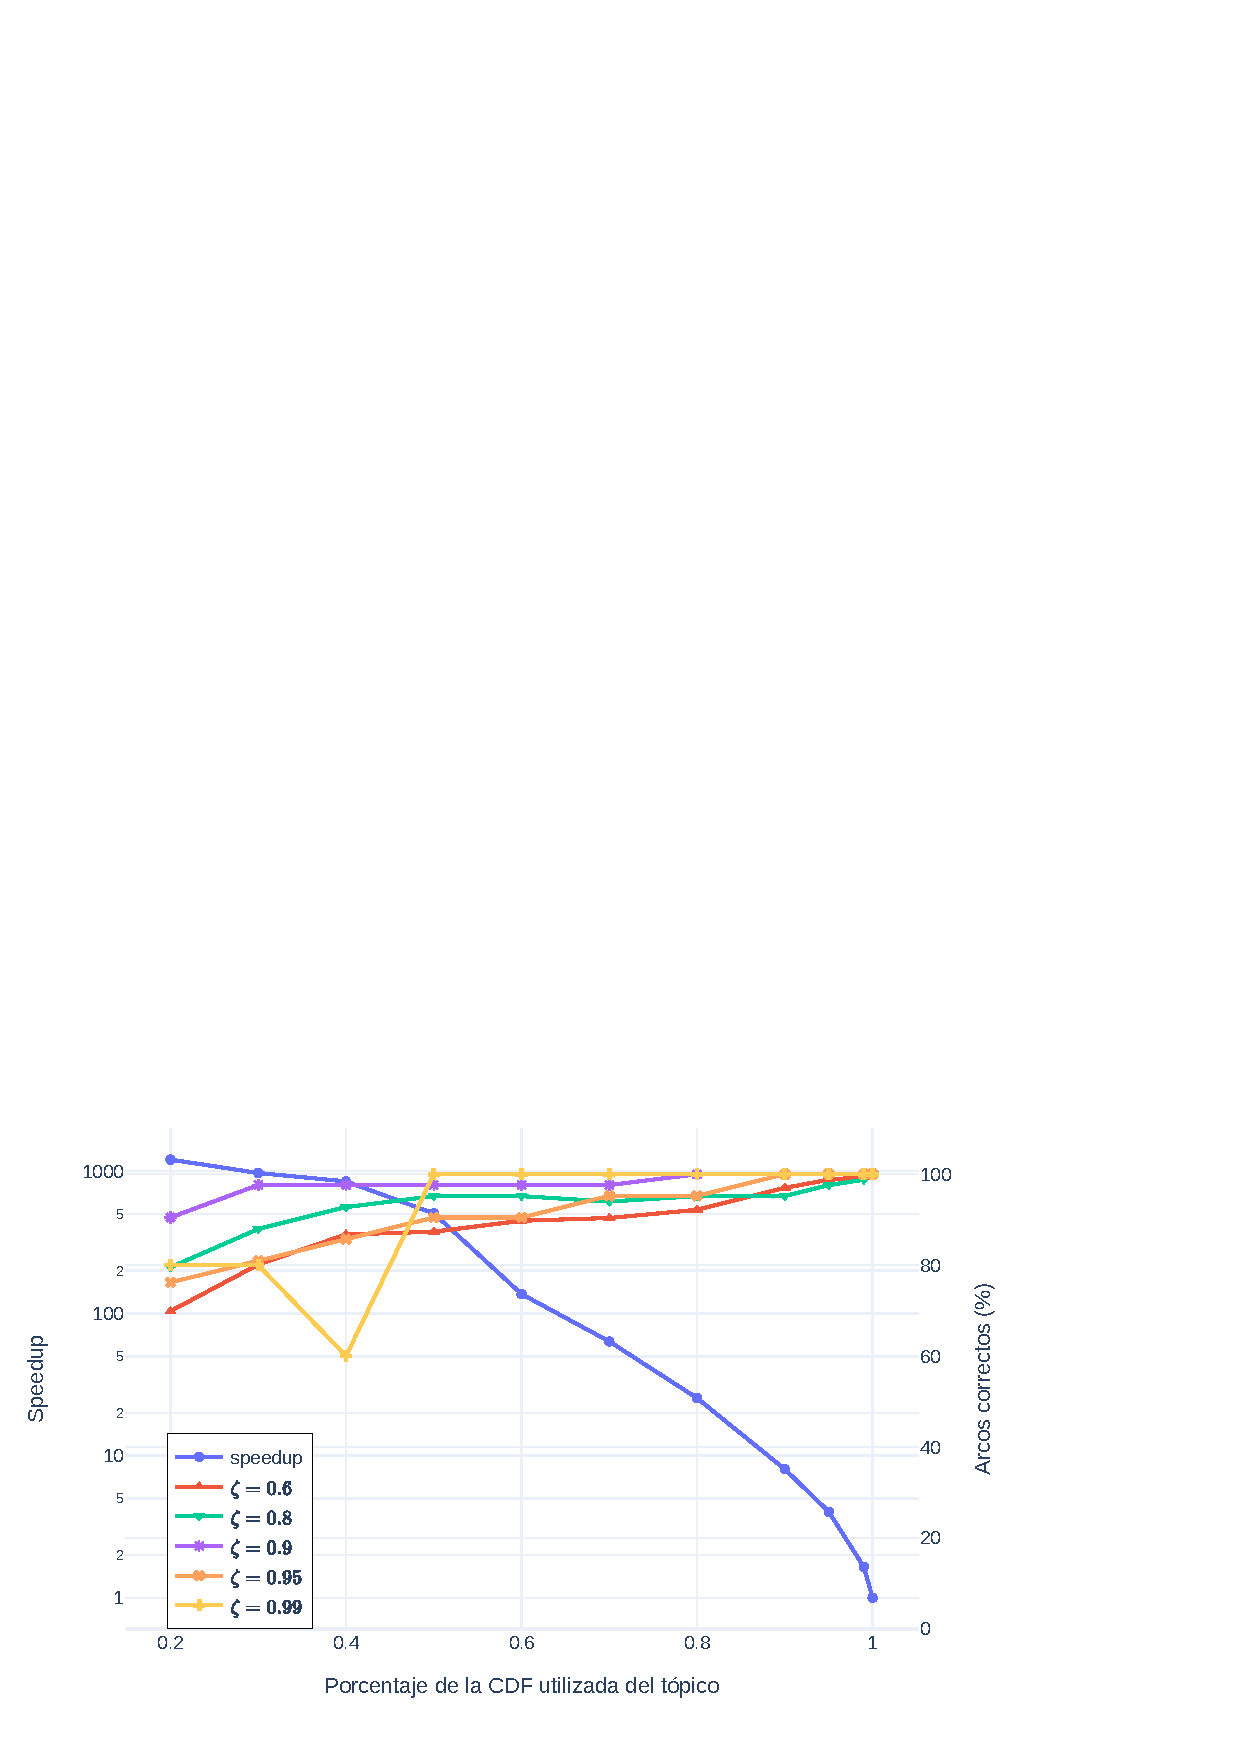
\includegraphics[width=1\textwidth]{ch3/speedup.png}
    \caption{Speedup promedio de la construcción del grafo en función de $q$. El speedup 1 equivale al tiempo más lento el cual está asciado a $q=0.95$ que es el valor de $q$ más grande y por ende con menor reducción de vocabulario de los tópicos a la hora de computar WMD.}
    \label{img:speedup}
\end{figure}\todoredo{Rehacer}

%\ref{img:ground_truth} y \ref{img:pruned_graph}
%conteo de arcos y blabla
%asociacion a tamaño de los topicos 
%no hablar todavía del significado de los tópicos

\begin{figure}
    \centering
    \includegraphics[width=0.8\textwidth]{ch3/ground_truth.png}
    \caption{Grafo temporal etiquetado.}
    \label{img:ground_truth}
\end{figure}\todoredo{Rehacer}

\begin{figure}
    \centering
    \includegraphics[width=0.8\textwidth]{ch3/pruned_graph.png}
    \caption{Grafo temporal obtenido a partir de la configuración óptima de parámetros $(q, \lambda, \zeta) = (0.2, 1.0, 0.9)$.}
    \label{img:pruned_graph}
\end{figure}\todoredo{Rehacer}

\section{Análisis cualitativo de resultados}
\todosec[inline]{Análisis cualitativo de tópicos}

\chapter{Conclusiones y trabajo futuro}
\todosec[inline]{Conclusiones}

\todosec[inline]{Otras aplicaciones}

\todosec[inline]{Trabajo futuro}

\bibliography{main}

% FIN DEL DOCUMENTO
\end{document}
